\setchapterpreamble[u]{\margintoc}
\chapter{System Analysis}
\labch{system-analysis}

In this chapter we present the analysis that was carried out in order to design all the components of the system.
Frist we sumarize the objectives and the components needed to meet those objectives. And after we will perform an
individual analysis for each one of the identified componenets with use cases and requirements.

\section{Objectives}
\labsec{ch04-objectives}

The objectives are those results that we want to achieve or features that we want the compiler to have once it is implemented. The main objectives that we have identified for the compiler are the following ones:
\begin{itemize}
    \item Provide the following tools from the compiler:
    \begin{itemize}
        \item Get the ST (syntax tree) from a source file.
        \item Get the AST (abstract syntax tree) from a ST.
        \item Get the SIL (ShEx-Lite Intermediate Language) from an AST.
        \item Generate sources in a given OOL from a SIL.
        \item For all the previos functionalities detect and inform or any event considered by the compiler as an error or warning.
    \end{itemize}
    \item Natively support, at least, Java and Python as target languages for the code generation.
    \item Allow the previous tools to be called from CLI.
    \item Allow the previous tools to be encapsulated in other programs written in any Java based language.
    \item Include examples of how the compiler works with a representative set of shape expressions.
\end{itemize}

\section{ShEx Based Syntax}
\labsec{ch04-shex-subset-analysis}

ShEx as itself it is not a syntax, it is a specification described in \sidecite{eric-rdf-validation-lang} 
and for that specification multiple syntaxes where proposed and implemented \sidecite{labra-validating-rdf}.
One of those syntaxes is the \texttt{Compact} syntax, which main goal is to be human frindly. It is also
the chossen one for IDE's and other tools that directly communicate with humans and therefore will be the
one that we will choose to start from.

As the title and the main goal of this project said this syntax needs to be a subset of ShEx, this is done
in order to allow \textbf{interoperability}, that is, every schema defined in this subset syntax needs to be
\textbf{fully compatible with other ShEx tools}.

In order to analyze all the features that our syntax will include we will perform some use cases and from
them we will extract the requirements that the syntax will need to implement.

\subsection{Syntax Use Cases}

\reffig{shex-lite-syntax-use-case} sows the high level view of the use cases that we expect ShEx-Lite syntax
to be use for. Those use cases include the \textbf{definition of prefixes}, the \textbf{definition of the base},
the \textbf{definition of the start shape expression} and the \textbf{definition of shape expressions}.

\begin{figure*}[h!]
	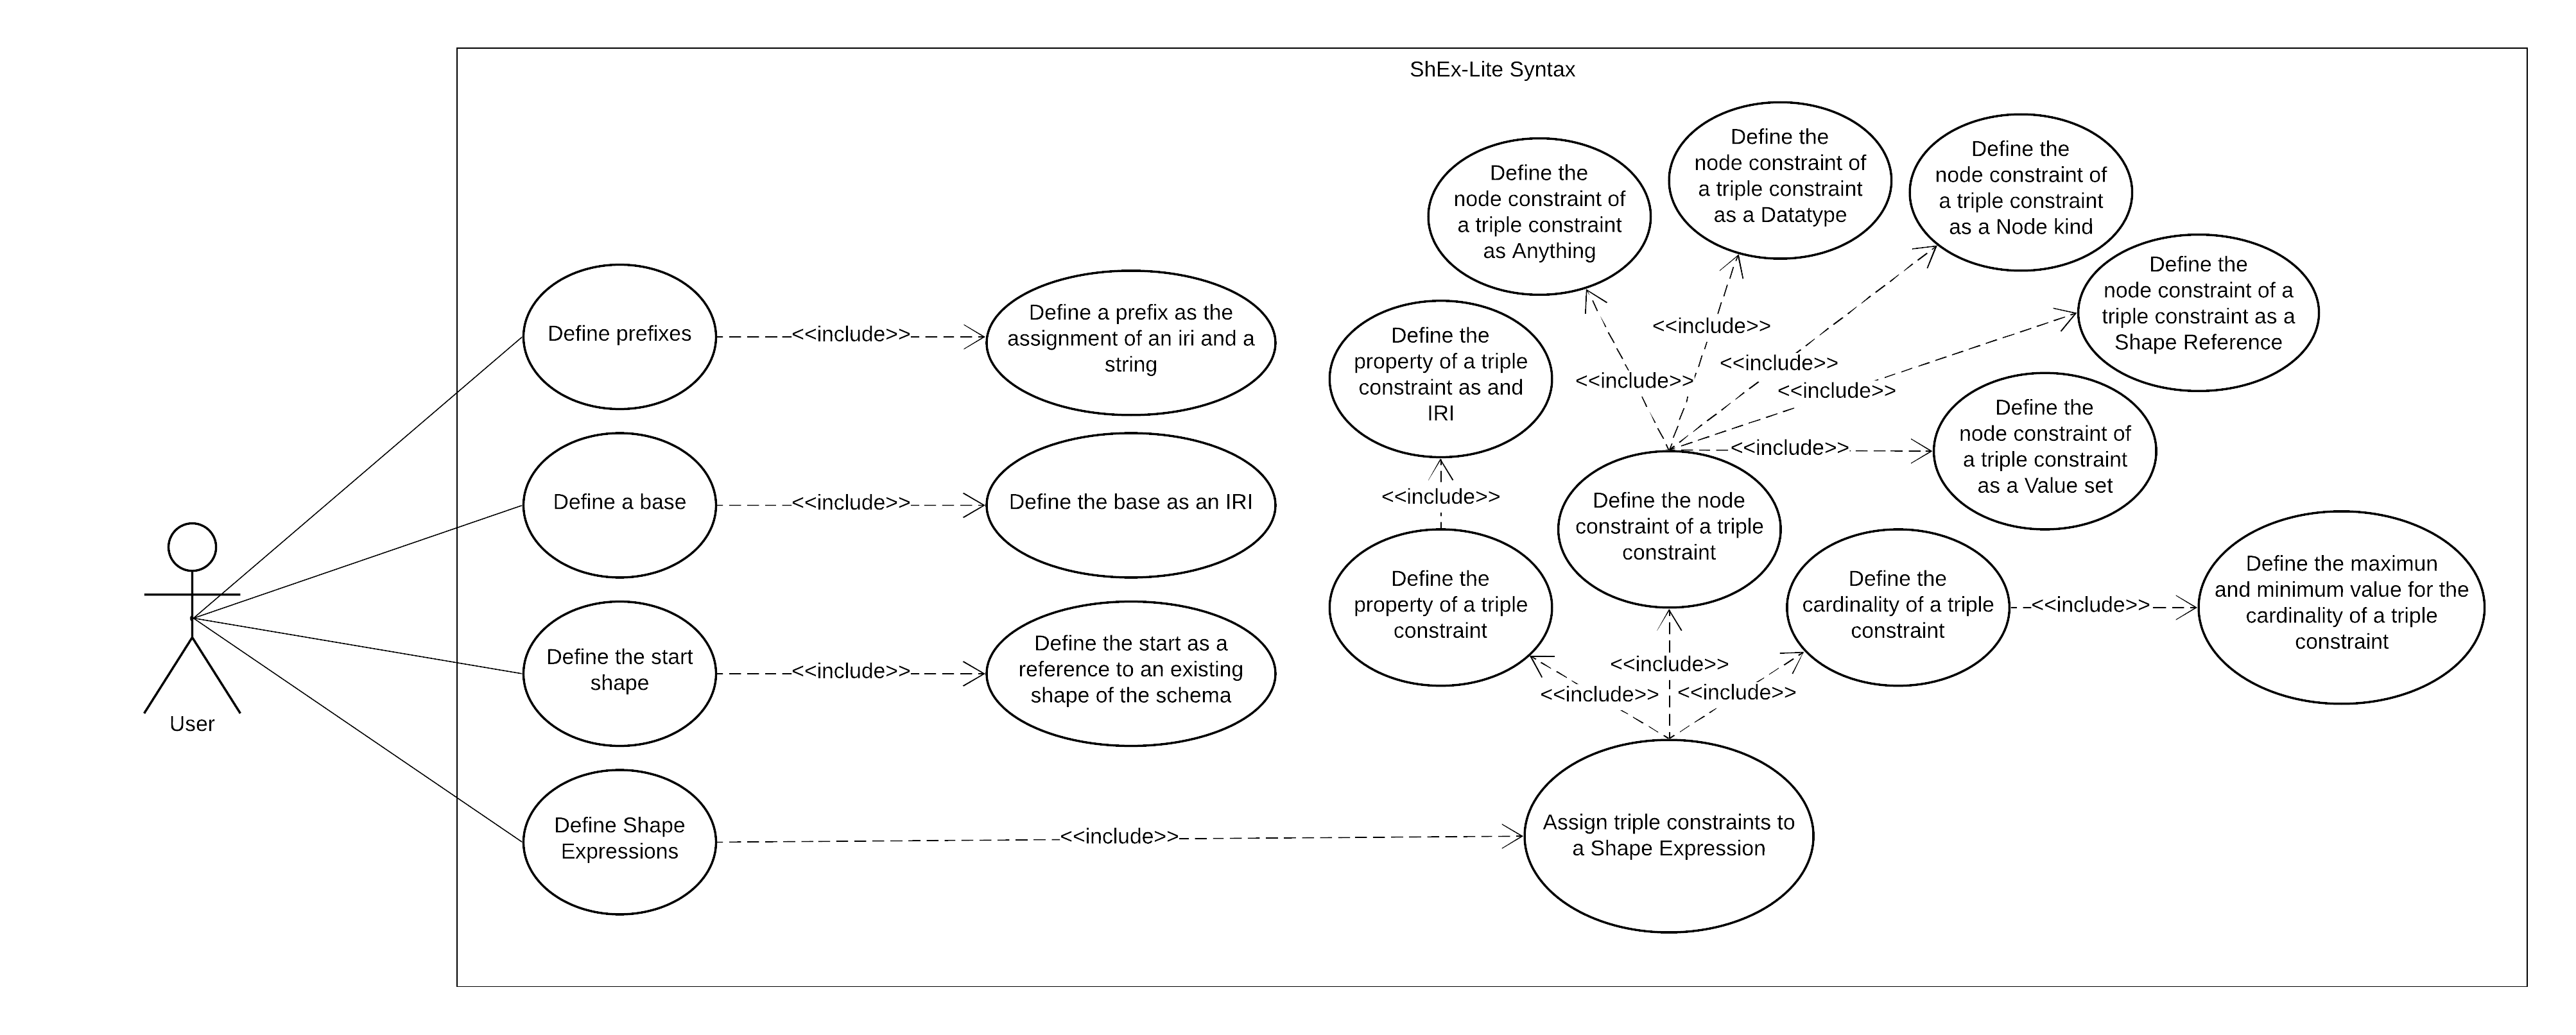
\includegraphics{shex-lite-syntax-use-case.png}
	\caption[ShEx-Lite syntax use case]{ShEx-Lite syntax use case.}
	\labfig{shex-lite-syntax-use-case}
\end{figure*}

Also the language will conservate most of the components of the shape expressions definitions from \texttt{ShEx}.
In our case a shape definition will be formed by a set of triple constraints. Each one of them will be of type
$Property$ $Constraint$ $Cardinality$.

\subsection{Syntax Requirements}
After we explore aims and the use cases that we expect for our syntax we can capture the requirements that grow
from them. It is important to remark that we are capturing the requirements of a syntax, not a system, therefore
we will only include the Syntax Requirements and the Quality Attributes that it must fullfil.

\subsubsection{Syntax Requirements}
The syntax requirements are those requirements that capture the functionality of the syntax, they will define
the actions that the syntax must allow to express.

\begin{enumerate}
    \item The syntax will allow to define prefixes.
    \begin{enumerate}
        \item A prefix definition will follow the ShEx specification.
    \end{enumerate}
    \item The syntax will allow to define a base.
    \begin{enumerate}
        \item A base definition will follow the ShEx specification.
    \end{enumerate}
    \item The syntax will allow to define the start shape expression.
    \begin{enumerate}
        \item The start shape expression will follow the ShEx specification.
    \end{enumerate}
    \item The system will allow to define shape expressions.
    \begin{enumerate}
        \item A shape expression will be formed by a shape label and a non-empty set of triple constraints.
        \begin{enumerate}
            \item A shape label will follow the ShEx specification.
            \item A triple constraint will be formed of the following elements:
            \begin{enumerate}
                \item The property. That will follow the ShEx specification.
                \item The node constraint. That will follow the ShEx specification.
                \item The cardinality. That will follow the ShEx specification.
            \end{enumerate}
        \end{enumerate}
    \end{enumerate}
\end{enumerate}

\subsubsection{Syntax Quality Attributes}
The syntax also includes some quality attributes that allow interoperability with other systems.
\begin{enumerate}
    \item The syntax will allow that any schema defined on it can be compiled by any other system that accepts ShEx Compact Syntax.
\end{enumerate}

\section{Compiler}
\labsec{ch04-compiler}

\section{Domain Object Models Generation}
\labsec{ch04-domg}

%\section{Target Users}
\labsec{ch04-target-users}

Every system has some target users, in the case of the SeX-Lite compiler we will focus it on three different types of users:
\begin{itemize}
    \item People with low technical skills that want to make schemas to validate RDF by means
    of shape expressions. This people will be able to compile their schemes and check for
    syntax / semantic errors or warnings through the CLI with a very simple instruction set.
    \item People with medium technical skills that want to transform a set of shape expressions
    in to a domain object model automatically. For this people the compiler will provide a
    manual that will explain each step of the transformation and an usage example.
    \item ShEx Community developers that want to test a new feature by implementing and
    testing its behaviors in a controlled small environment. For this people the compiler
    provides not only the public API but the source code and the corresponding technical
    documentation. 
\end{itemize}

%\section{Use Cases}
\labsec{ch04-use-cases}

The first stage to analyze our system is to see the use cases view, from there we will try to capture posible requirements and with all that information design our system.

\begin{figure}[hb]
    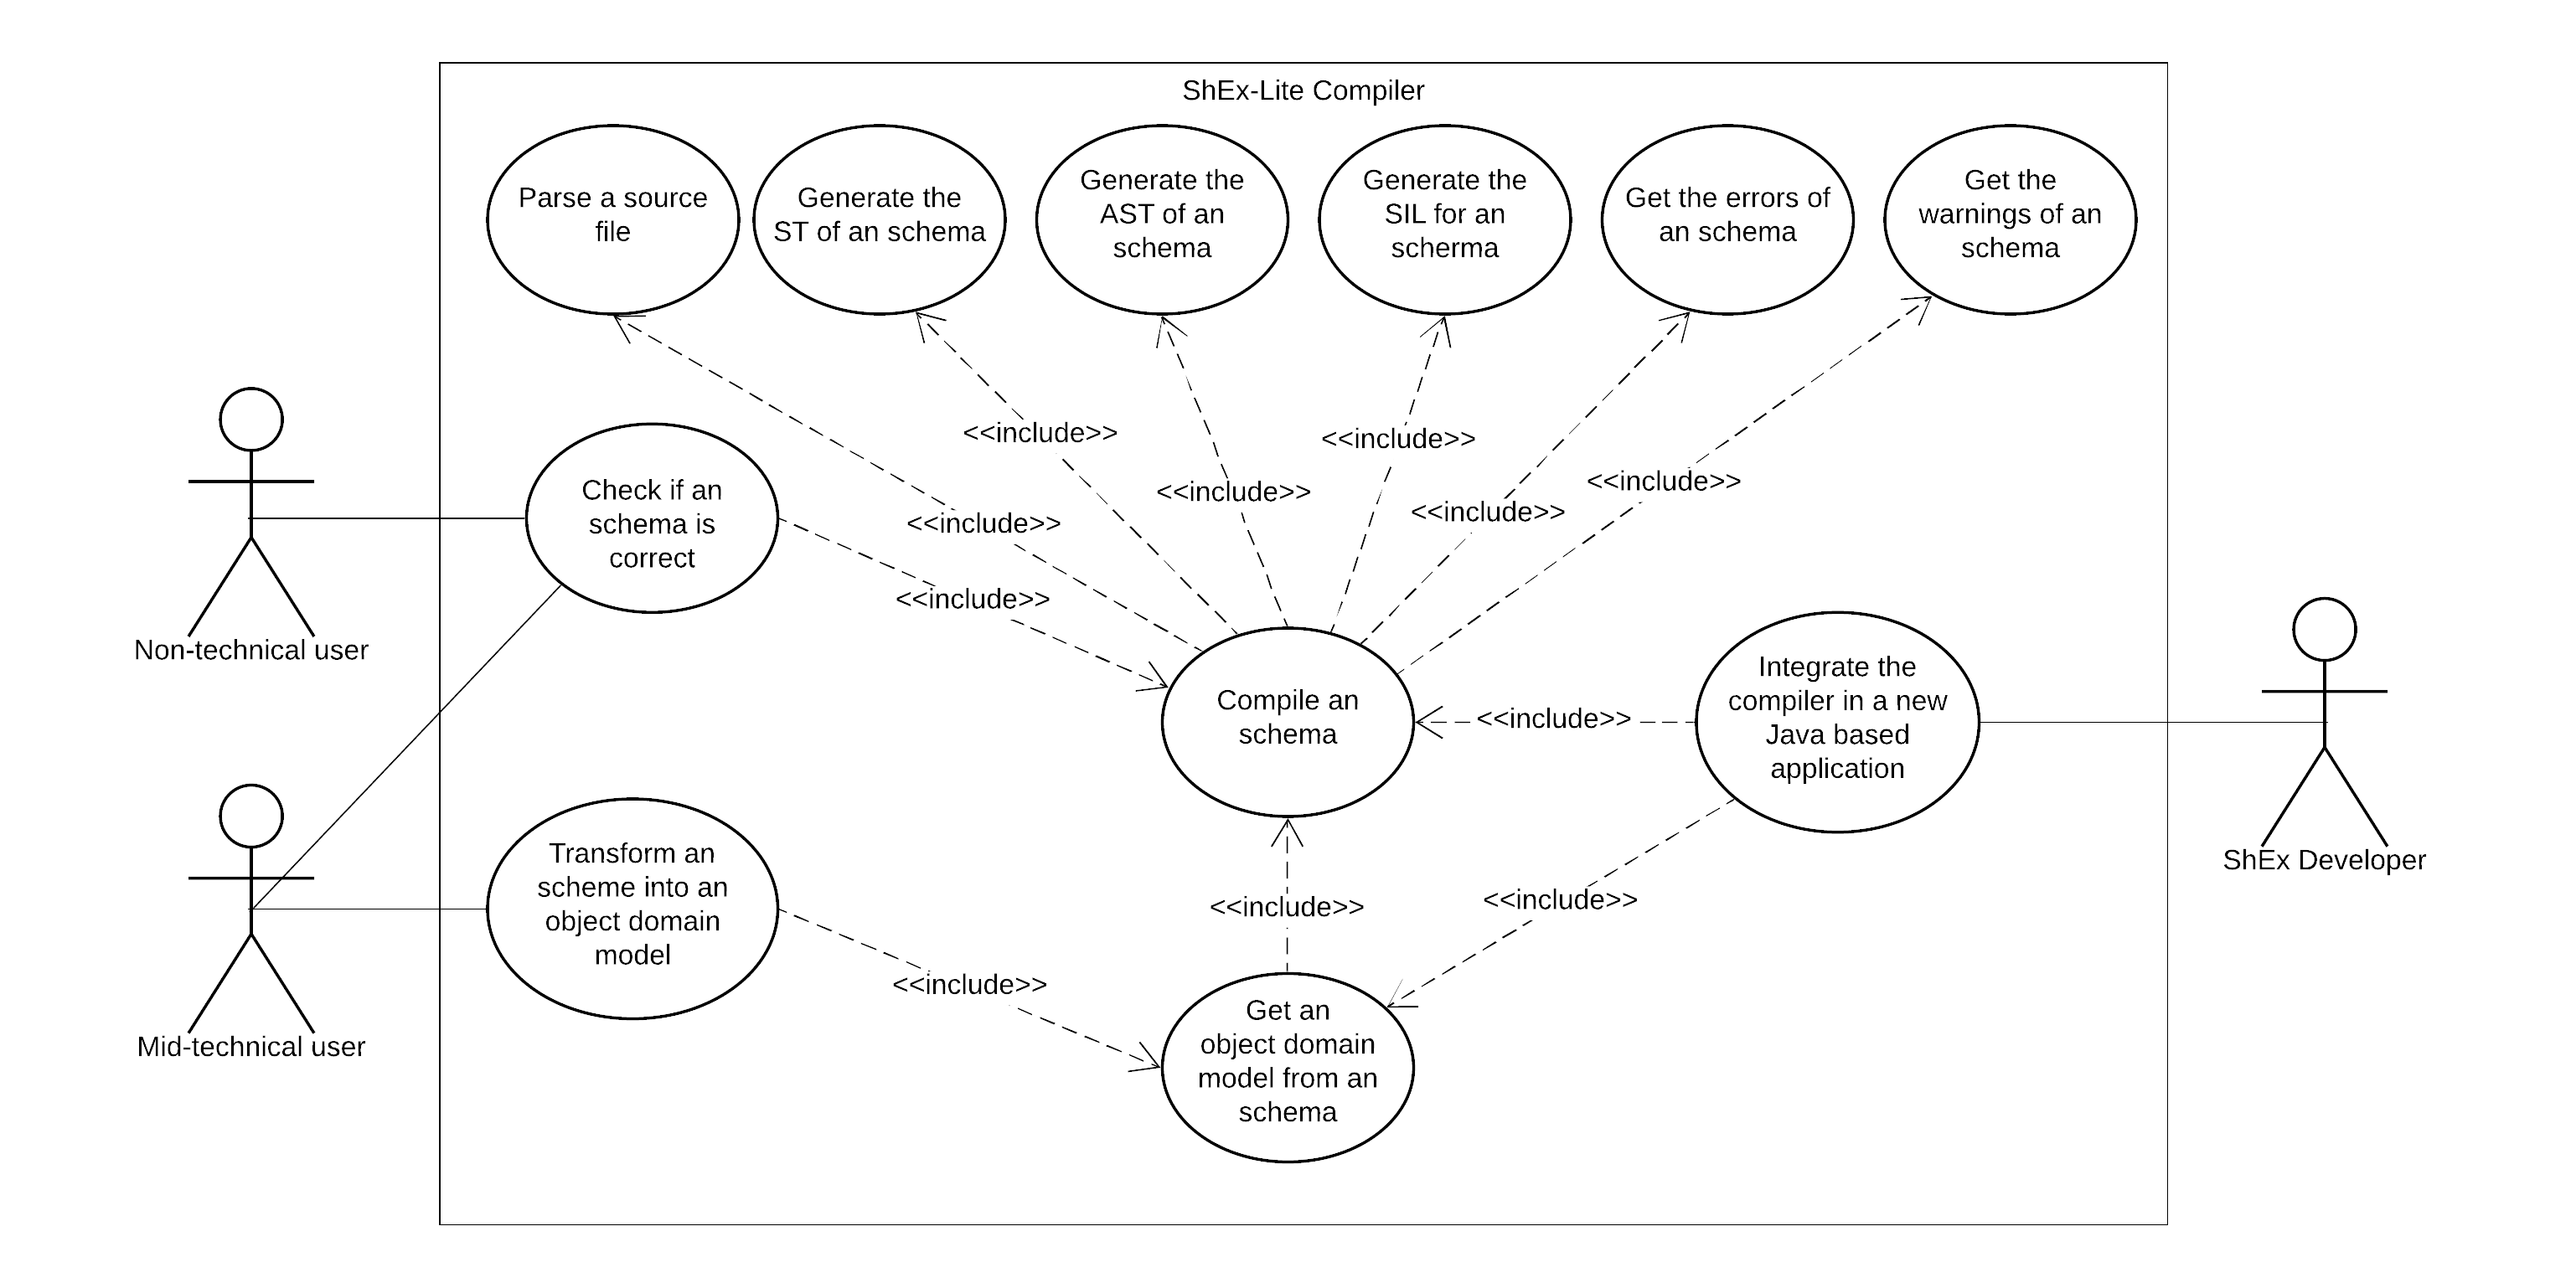
\includegraphics{shex-lite-use-cases-01.png}
    \caption[Use cases view of the ShEx-Lite compiler for the three different actors of the system]{Use cases view of the ShEx-Lite compiler for the three different actors of the system.}
    \labfig{shex-lite-use-cases-01}
\end{figure}

In \reffig{shex-lite-use-cases-01} we can see the high level view of the different use cases that the three different target users of the systems might have, now we will analyze each one individually, some the internal use cases that have no direct interaction with the target user will be explored after.

\subsection{Non technical user}
The non technical target user is intended to use only the compiler to validate if the schemas they have defined are syntactically and semantically correct, or if they have any error or warning to be aware of them. \reffig{shex-lite-use-cases-02} shows the interaction diagram for this actor, and \reftab{use-case-01-tab} describes the represented use case.

\begin{figure}[hb]
    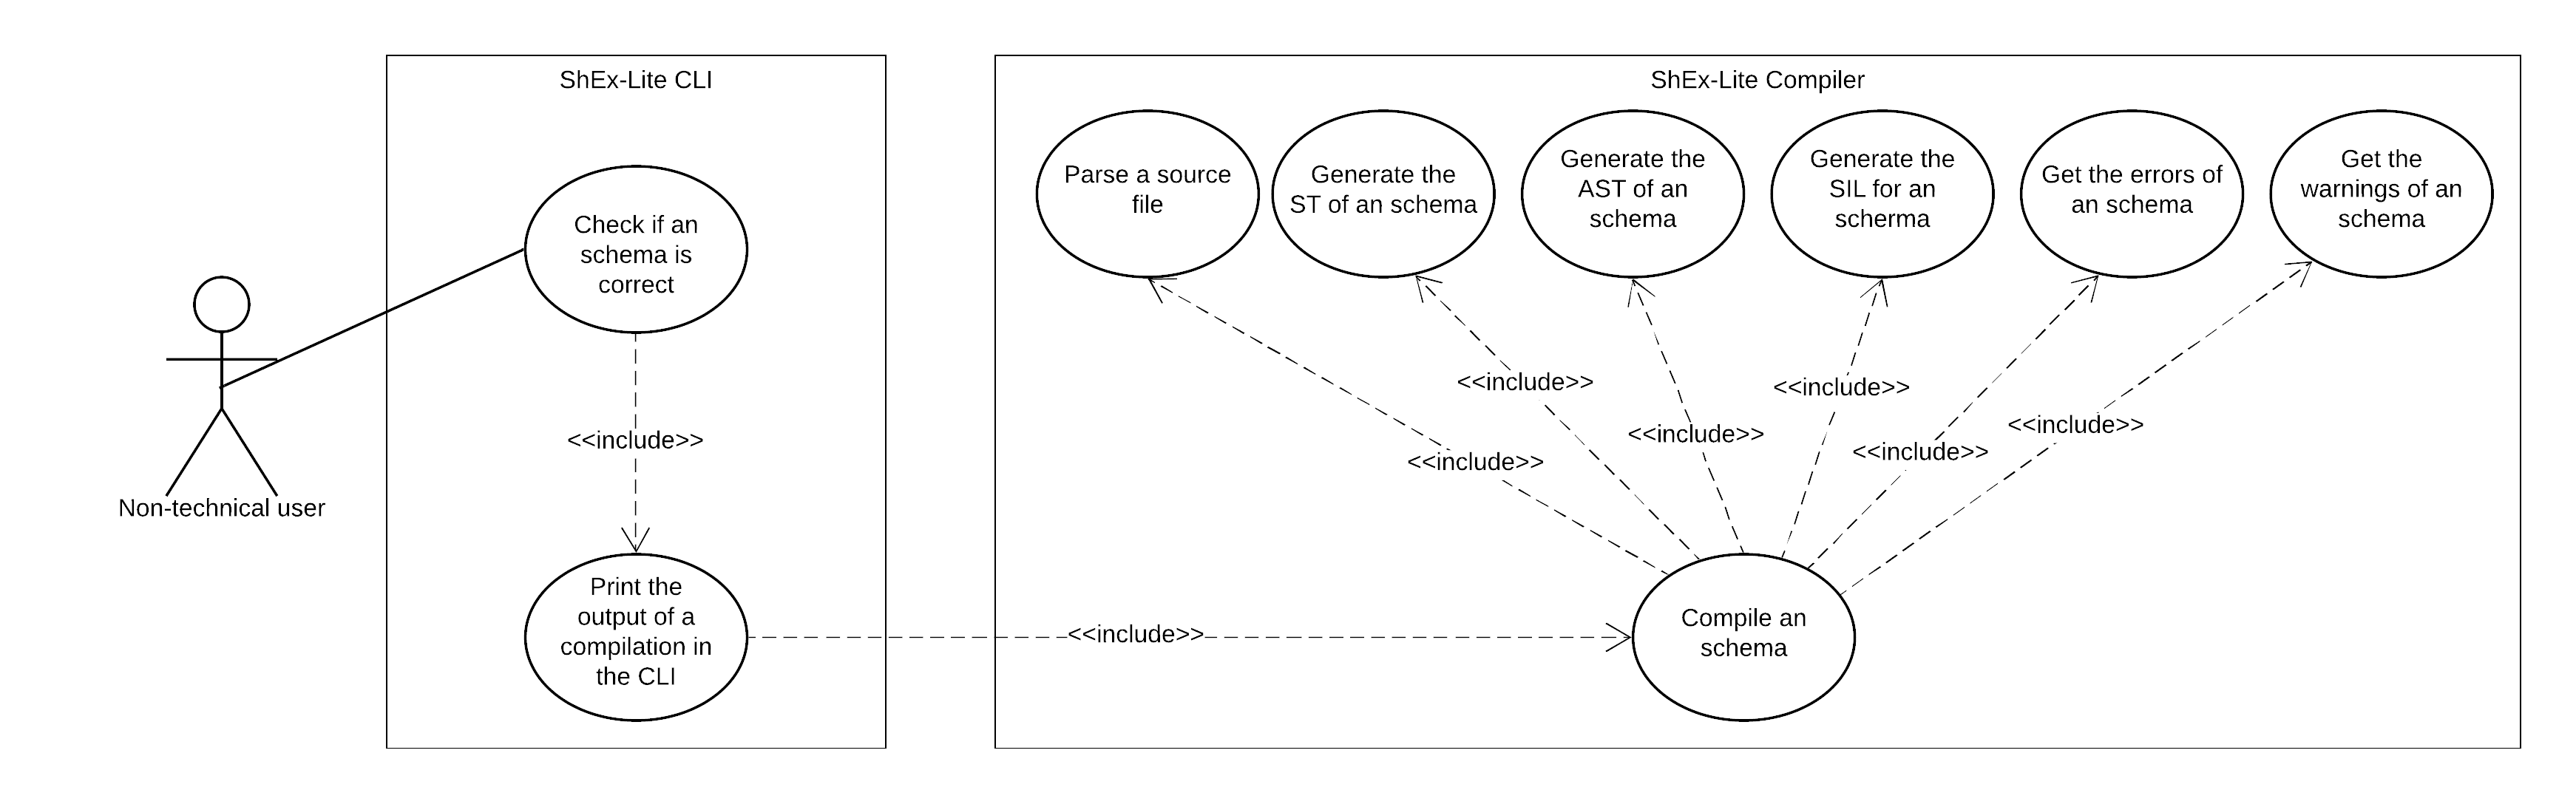
\includegraphics{shex-lite-use-cases-02.png}
    \caption[Extension of the use case view for a non technical user]{Extension of the use case view for a non technical user.}
    \labfig{shex-lite-use-cases-02}
\end{figure}

\begin{table}
    \begin{tabular}{ | m{2cm} | m{8cm}| }
        \toprule
        Use Case Number & 1 \\
        \midrule
        Description & Check if an schema is correct from the CLI tool. \\
        \midrule
        Actor & Non technical user. \\
        \midrule
        Flow & The actor wants to check if schema is correct or not. If it is not correct wants to see all the warnings / errors. For this purpose the actor introduces the schema in the CLI tool and starts the flow. Once the flow is complete the actor wants to see information that helps to decide if the schema is correct or not. \\
        \bottomrule
    \end{tabular}
    \caption[Definition of the use case number 1 for the non technical user]{Definition of the use case number 1 for the non technical user.}
    \labtab{use-case-01-tab}
\end{table}

\subsection{Mid technical user}
The use cases expected for a mid technical user are two, in one side the compilation in order to validate if their schemas are syntactically and semantically correct, or if they have any error or warning. And on the other hand, automatically generate the domain object models for the defined schema. For this user we can find the representation of the interaction diagram at \reffig{shex-lite-use-cases-03} and both associated use cases descriptions on \reftab{use-case-02-tab} and \reftab{use-case-03-tab}.

\begin{figure}[hb]
    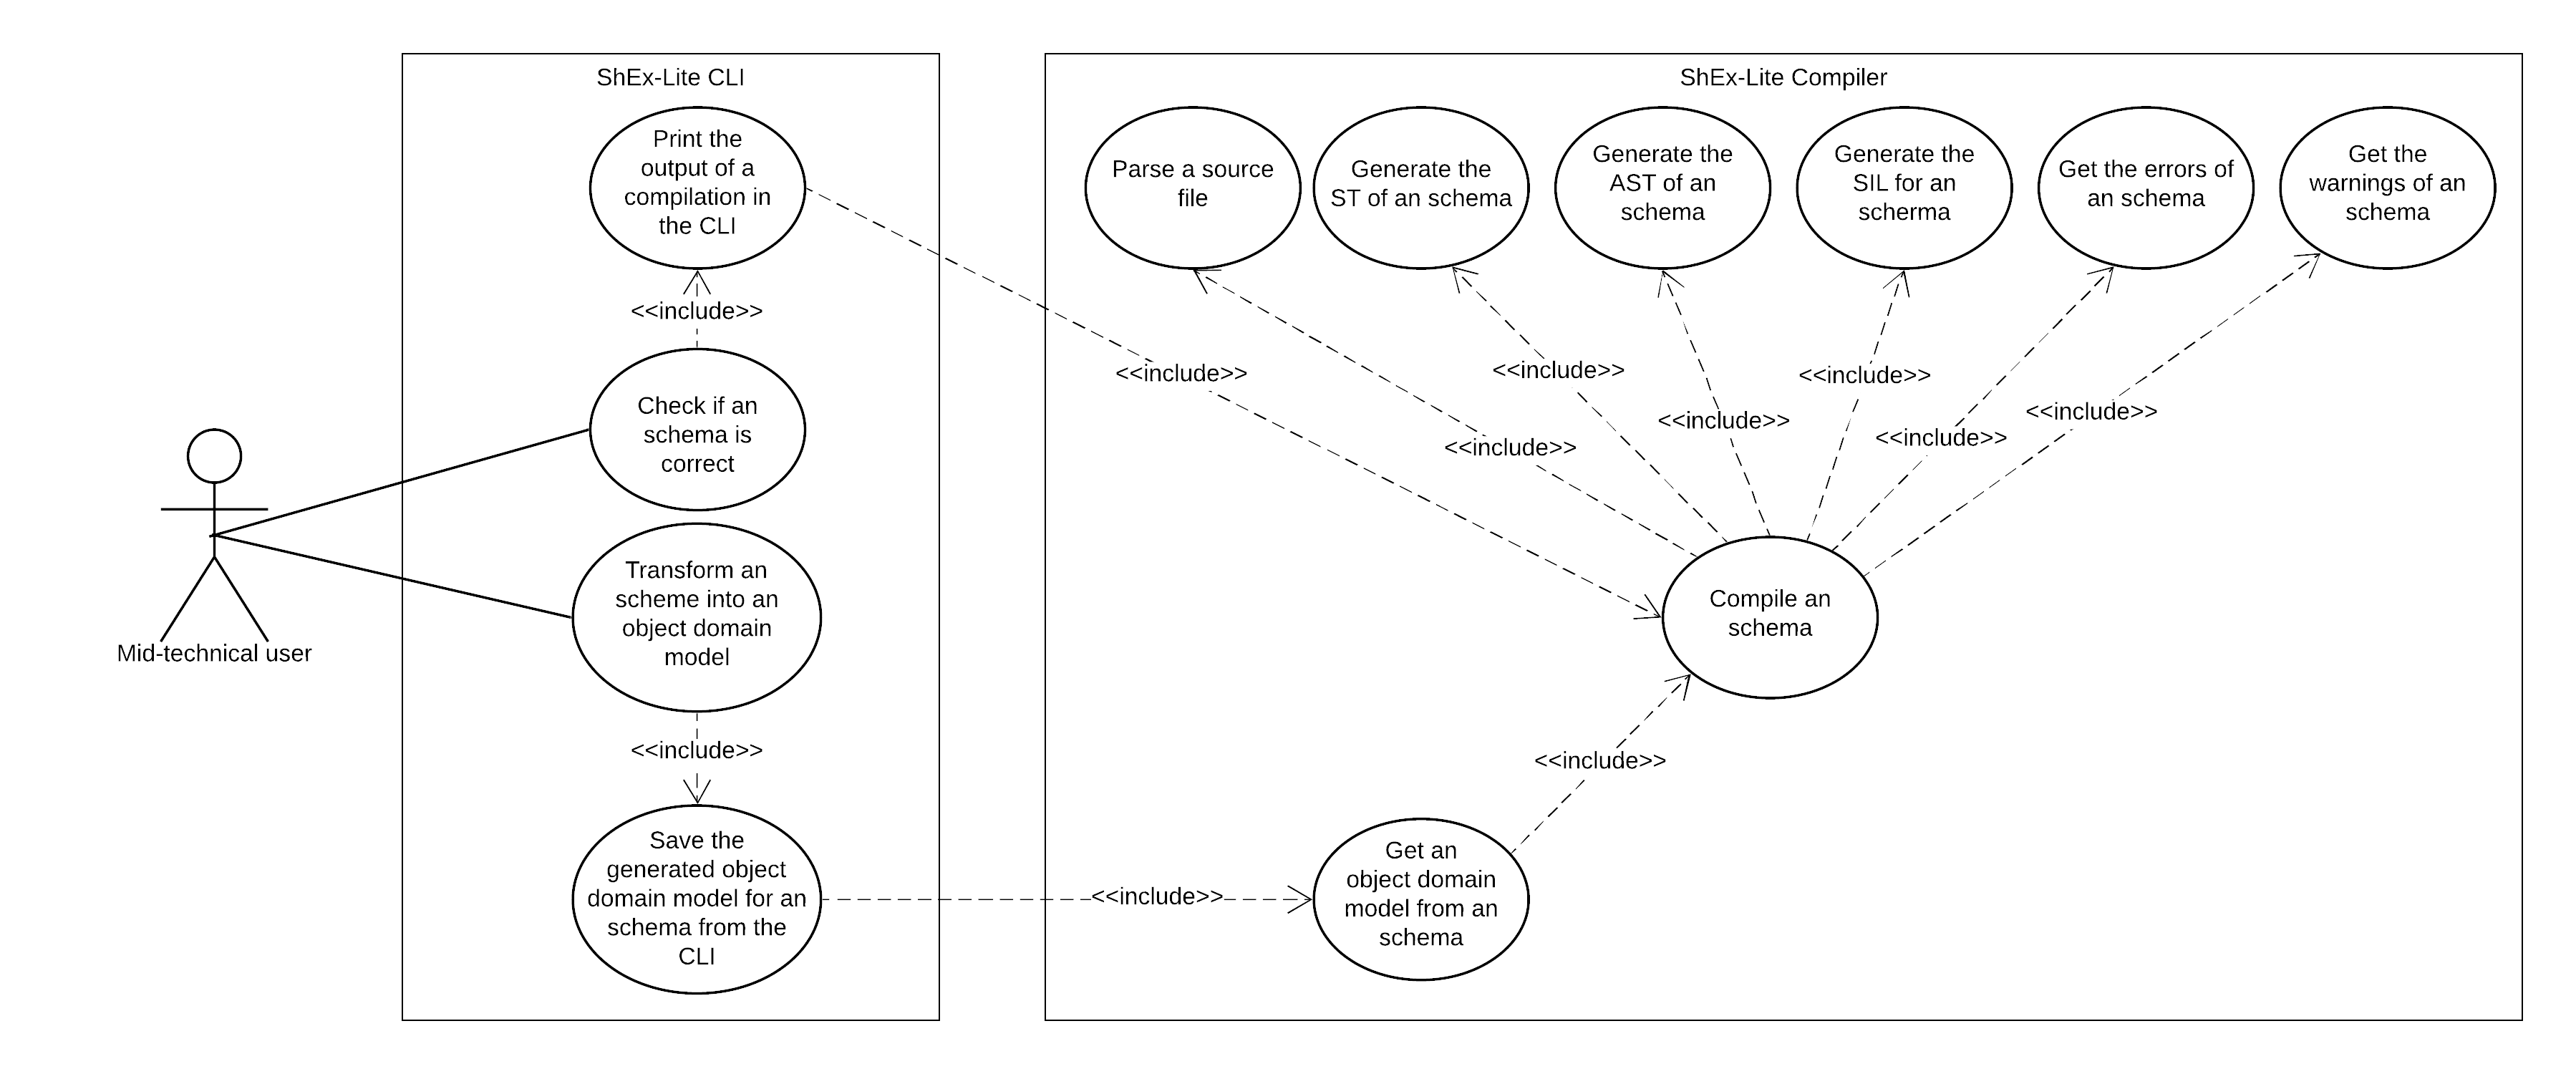
\includegraphics{shex-lite-use-cases-03.png}
    \caption[Extension of the use case view for a mid technical user]{Extension of the use case view for a mid technical user.}
    \labfig{shex-lite-use-cases-03}
\end{figure}

\begin{table}
    \begin{tabular}{ | m{2cm} | m{8cm}| }
        \toprule
        Use Case Number & 2 \\
        \midrule
        Description & Generate an object domain model for a given schema from the CLI. \\
        \midrule
        Actor & Mid technical user. \\
        \midrule
        Flow & The actor wants to generate an object domain model for a given schema from the CLI tool. For this purpose the actor introduces the schema in the CLI tool and starts the flow. Once the flow in complete the actor wants the generated object model to be persist as source files on his computer. \\
        Conditions & For this flow to end correctly it is mandatory that the schema that the user uses to generate the domain object model is correct. \\
        \bottomrule
    \end{tabular}
    \caption[Definition of the use case number 2 for the mid technical user]{Definition of the use case number 2 for the mid technical user.}
    \labtab{use-case-02-tab}
\end{table}

\begin{table}
    \begin{tabular}{ | m{2cm} | m{8cm}| }
        \toprule
        Use Case Number & 3 \\
        \midrule
        Description & Check if an schema is correct from the CLI tool. \\
        \midrule
        Actor & Mid technical user. \\
        \midrule
        Flow & The actor wants to check if schema is correct or not. If it is not correct wants to see all the warnings / errors. For this purpose the actor introduces the schema in the CLI tool and starts the flow. Once the flow is complete the actor wants to see information that helps to decide if the schema is correct or not. \\
        \bottomrule
    \end{tabular}
    \caption[Definition of the use case number 3 for the mid technical user]{Definition of the use case number 3 for the mid technical user.}
    \labtab{use-case-03-tab}
\end{table}

\subsection{ShEx Developer}
A ShEx developer is expected to use the compiler in two ways, first to integrate it in to other applications and secondly to generate object domain models for a given schema but not from the CLI, from an API instead. \reffig{shex-lite-use-cases-04} shows the interaction diagram of this actor with the compiler and \reftab{use-case-04-tab} descrives this use case scenario.

\begin{figure}[hb]
    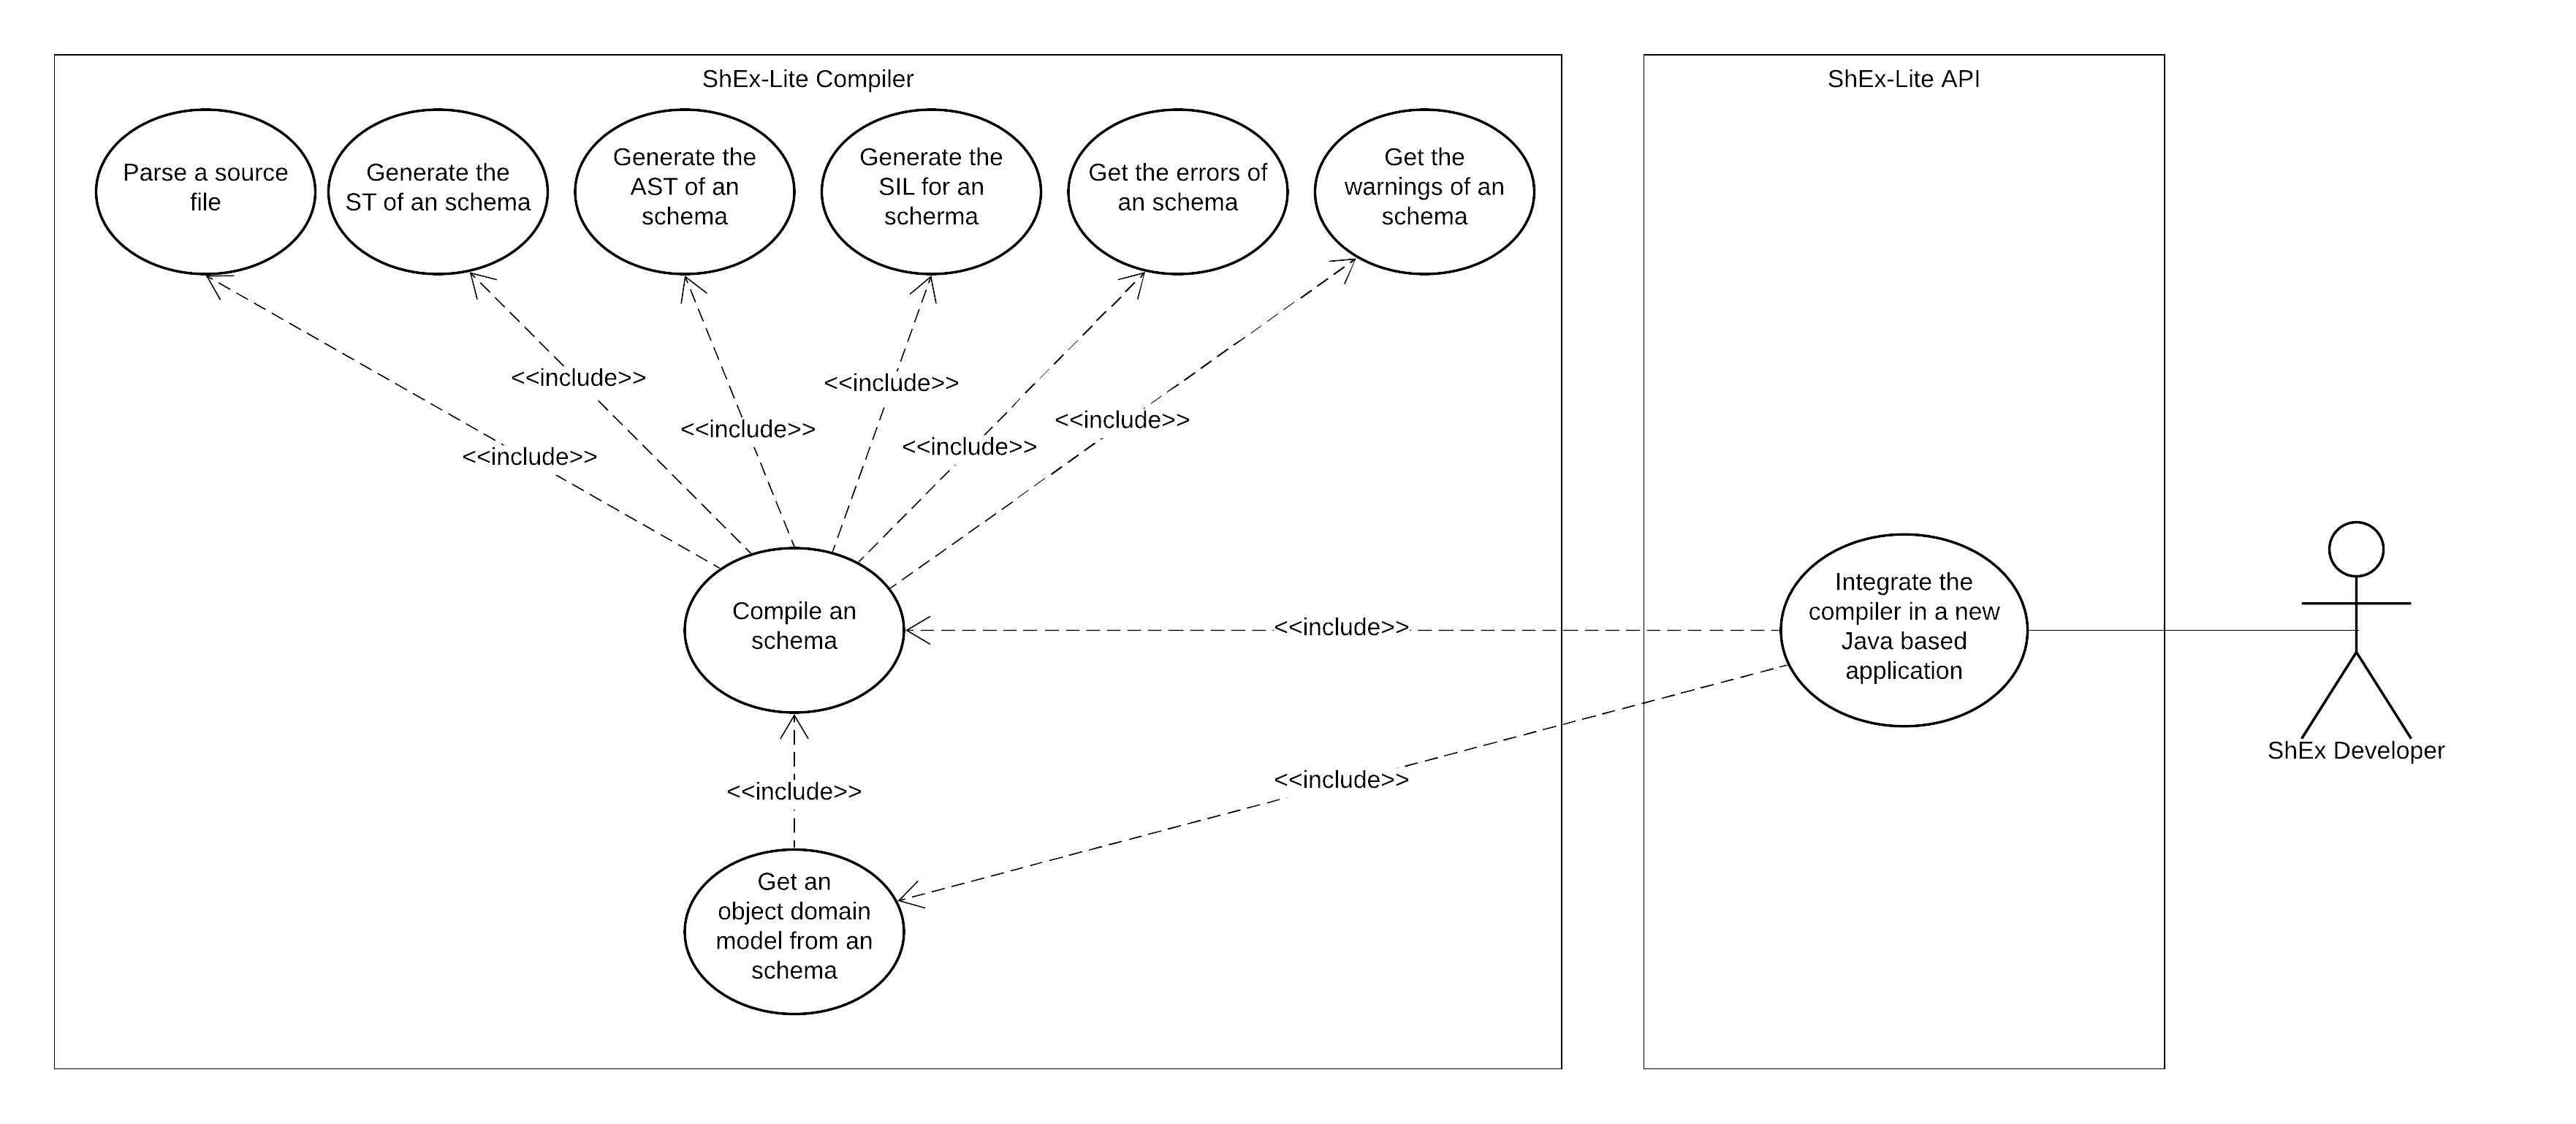
\includegraphics{shex-lite-use-cases-04.png}
    \caption[Extension of the use case view for a mid technical user]{Extension of the use case view for a mid technical user.}
    \labfig{shex-lite-use-cases-04}
\end{figure}

\begin{table}
    \begin{tabular}{ | m{2cm} | m{8cm}| }
        \toprule
        Use Case Number & 4 \\
        \midrule
        Description & Integrate the compiler in a new Java based application. \\
        \midrule
        Actor & ShEx developer. \\
        \midrule
        Flow & The actor wants to integrate the compiler in to a new java base application. For that purpose the actor will use a public API that allow the actor to integrate the actions described in the use cases 2 and 3. \\
        \bottomrule
    \end{tabular}
    \caption[Definition of the use case number 4 for the ShEx developer user]{Definition of the use case number 4 for the ShEx developer user.}
    \labtab{use-case-04-tab}
\end{table}

\bigskip
The previous use cases might seem like the system is really simple, but far from truth the
fact that the interface with the target users is simple does not define the complexity of the
system, as this, lives inside of it. In order to capture this complexity we will proceed now to
analyze the requirements that the implemented system must meet. 

%\section{Requirements}
\labsec{ch04-requirements}

In this section we are going to enumerate the requirements that we have obtained for the
compiler. Since the line that separates functional and non-functional requirements can be
sometimes hard to define, we decided to specify the requirements following the taxonomy
introduced in the IEEE 830 standard for the specification of software requirements. The
following types of requirements will be evaluated:

\begin{itemize}
    \item External interfaces: Requirements that affect user, hardware, software or communication interfaces.
    \item Functional requirements: Requirements related to the functions of the system.
    \item Performance requirements: These requirements are related to the load that the system should tolerate.
    \item Logical database requirements: These requirements are related to access or constraints with the system’s database.
    \item Design constraints: Constraints imposed by standards, hardware limitations…
    \item Other constraints.
    \item System attributes: Quality attributes of the system, such as usability, accessibility…
    \item Other requirements that do not belong to any of the categories above.
\end{itemize}

\subsection{External Interfaces}

\subsection{Functional Requirements}

\subsection{Performance Requirements}

\subsection{Design Constraints}

\subsection{Other Constraints}

\subsection{System Attributes}

\subsection{Other Requirements}


%\section{Identified Subsystems}
\labsec{ch04-subsystems}

Once the definition of the scope was finished, and the requirements were captured and documented, the following subsystems were identified.

\subsection{Compiler}
The compiler subsystem, called shexlc includes all the necessary elements to validate that
an schema is correct, or provide with the necessary information to fix any error it might
contain. And generate domain object models for the correct schemas. 

\subsection{CLI tool}
The CLI Tool provide both non technical and mid technical users the ability to use the
compiler from a text interface, allowing them to validate syntactically and semantically the
schemas. This validation involves also informing if any error or warning is generated during
the compilation. And in the case mid technical users also it provides the ability to generate
domain object models by saving them in the computer as source files. 

\subsection{Public API}
The compiler public API, called shexl, provides to the ShEx Community developers the
ability to access the different stages of the compilation process independently. Its main
objective is to provide them with a simple API that allows them not only to integrate the
compiler on different applications but also to extend it easily. 